\section{Adjusting the Parameters}
\label{sec:add.parameters}

The fixed parameters in the archetypal are $a_L = 4, b_L = -\frac{1}{2},$ and $g_R\left(\frac{1}{2}\right) = \frac{1}{2} + \frac{1}{40}$.
\hl{O}nly the branches $f_\A$ and $f_\C$ are not monotonously increasing.
Of the three fixed parameters, $a_L$ and $b_L$ influence the shape of the branches $f_\A$ and $f_\C$.
\hl{These parameters are adjusted to make the branches $f_\A$ and $f_\C$ monotonously increasing}.
The new parameter values are $a_L = 1$ and $b_L = \frac{1}{2}$.
The new shape of the function can be seen in \Cref{fig:add.arch.new}, now all branches are monotonously increasing.
And \Cref{add.arch.new.period} shows a 2D scan of the periods associated with parameter regions in the archetypal model with these new values for the fixed parameters.

\begin{figure}
	\centering
	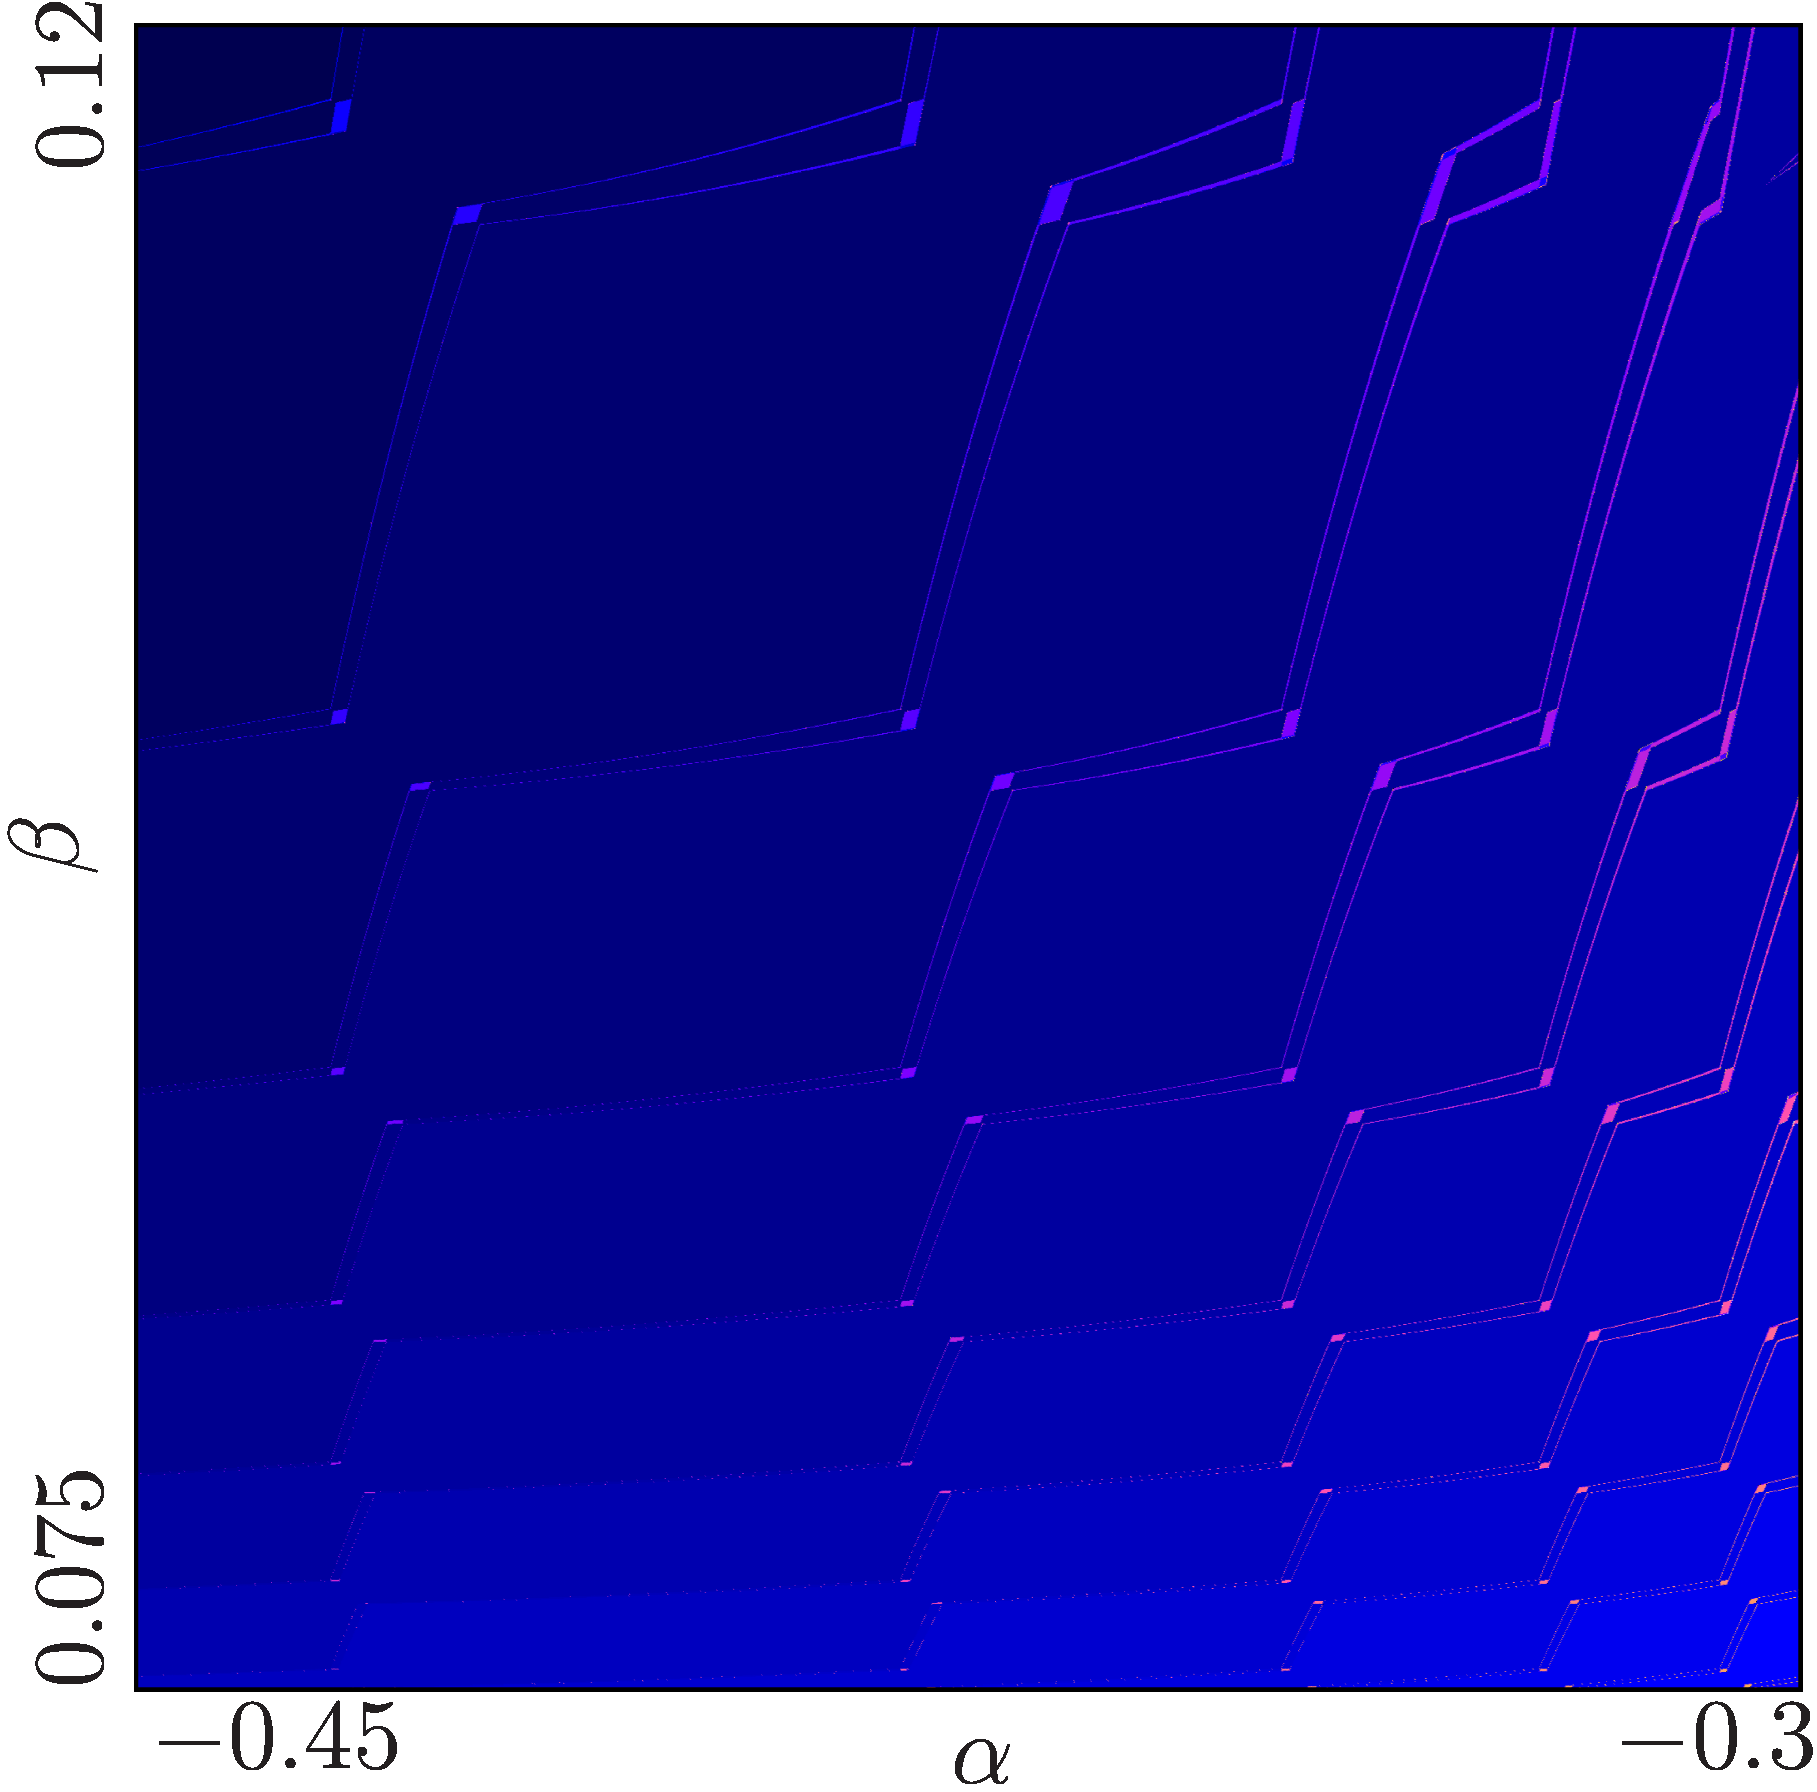
\includegraphics[width=.7 \textwidth]{../Figures/7/7.1/result.png}
	\caption[2D period scan of the piecewise-increasing increasing archetypal model]{
		2D period scan of the piecewise-increasing increasing archetypal model.
		With the fixed parameters $a_L = 1, b_L = \frac{1}{2},$ and $g_R\left(\frac{1}{2}\right) = \frac{1}{2} + \frac{1}{40}$.
		The parameters $\alpha = g_R\left(\frac{1}{4}\right)$ and $\beta = c_L$ are varied.
	}
	\label{fig:add.arch.new.period}
\end{figure}

\todo{Rewrite rest of this section}

We will refer to this model as the increasing archetypal model.
In this scan, we can see that the ``type B'' parameter regions disappeared and ``type A'' parameter regions of the same chain seem to start overlapping.
Also, in between the chains there are now small parameter regions with much higher periods.
This looks like period-adding, and we will explore it in the following sections.
But first, we will take a closer look at how the bifurcations structures change when adjusting the parameters $a_L$ and $b_L$ to make the branches $f_\A$ and $f_\C$ increasing.

\todo{Explanation: old}

It was shown that there are period-adding structures in piecewise linear continuous increasing circle maps by \Citeauthor{simpson2018saw}.
He calls these types of functions skew sawtooth maps~\cite{simpson2018saw}.
The archetypal model function is not continuous, has four branches instead of two, and only linear on two of four branches.
But it is also a circle map, \gls{pws}, and mostly increasing.
\Cref{fig:add.saw.vs.arch} shows both maps for comparison.
In this chapter, we modify the fixed parameters of the archetypal model to produce period-adding structures.
The idea is to make the archetypal model function as similar as possible to a skew sawtooth map.

\begin{figure}
	\centering
	\subfloat[Skew sawtooth map]{
		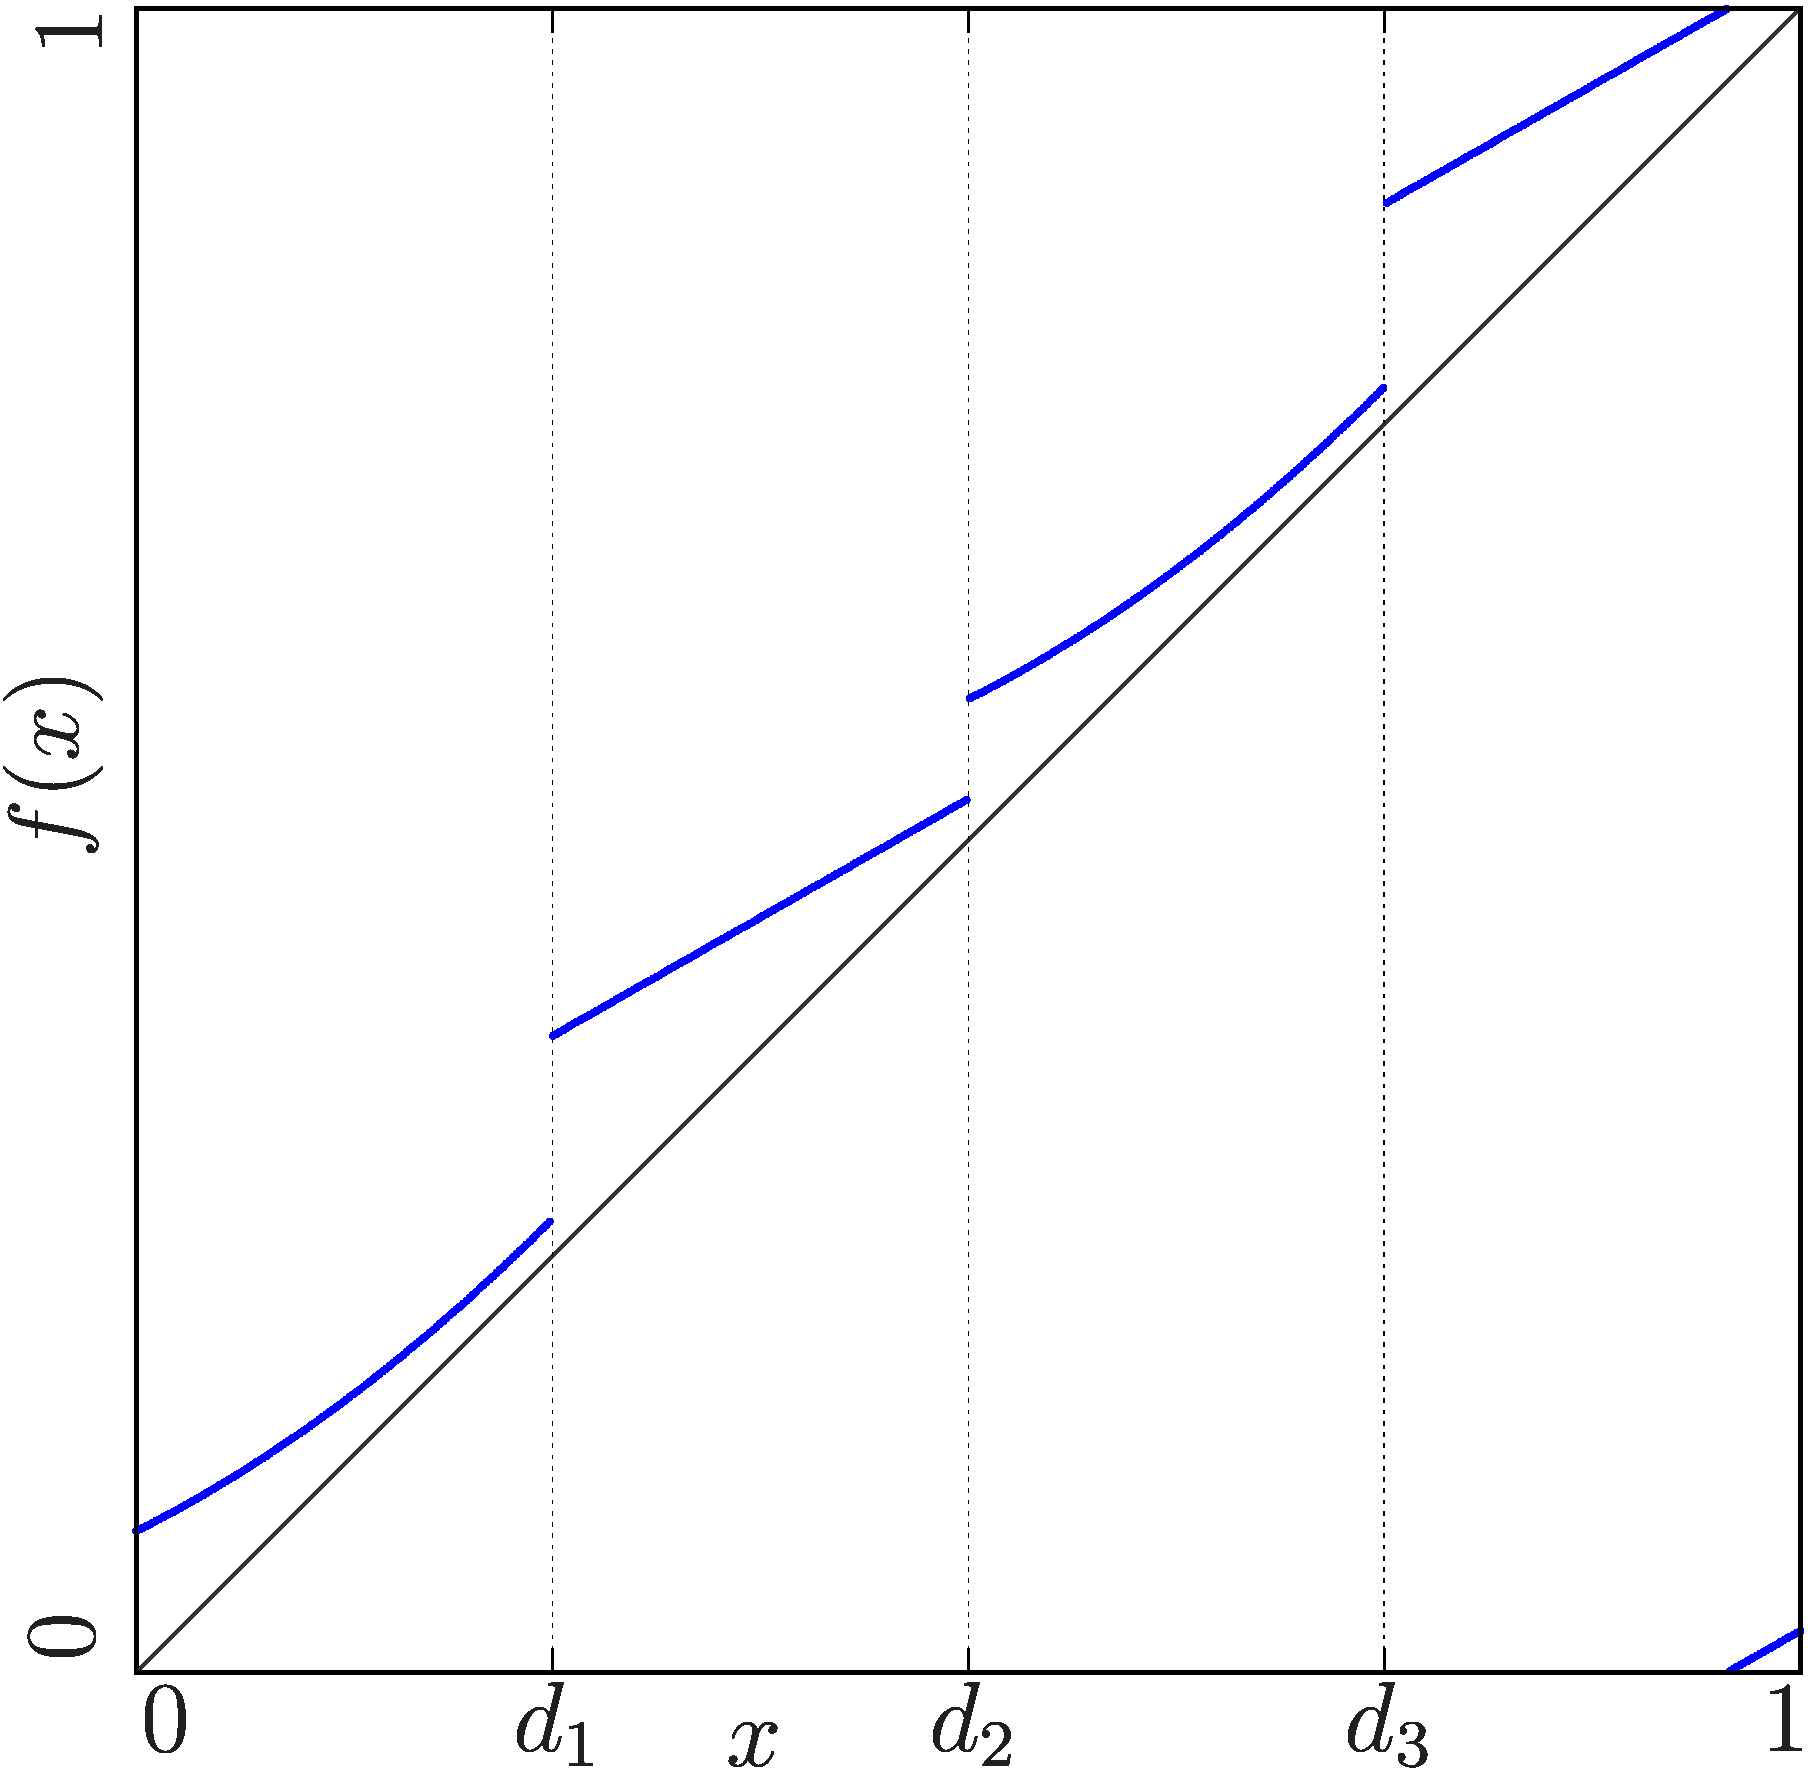
\includegraphics[width=.45 \textwidth]{../Figures/7/7.2a/result.png}
		\label{fig:add.saw}
	}
	\subfloat[Function shape]{
		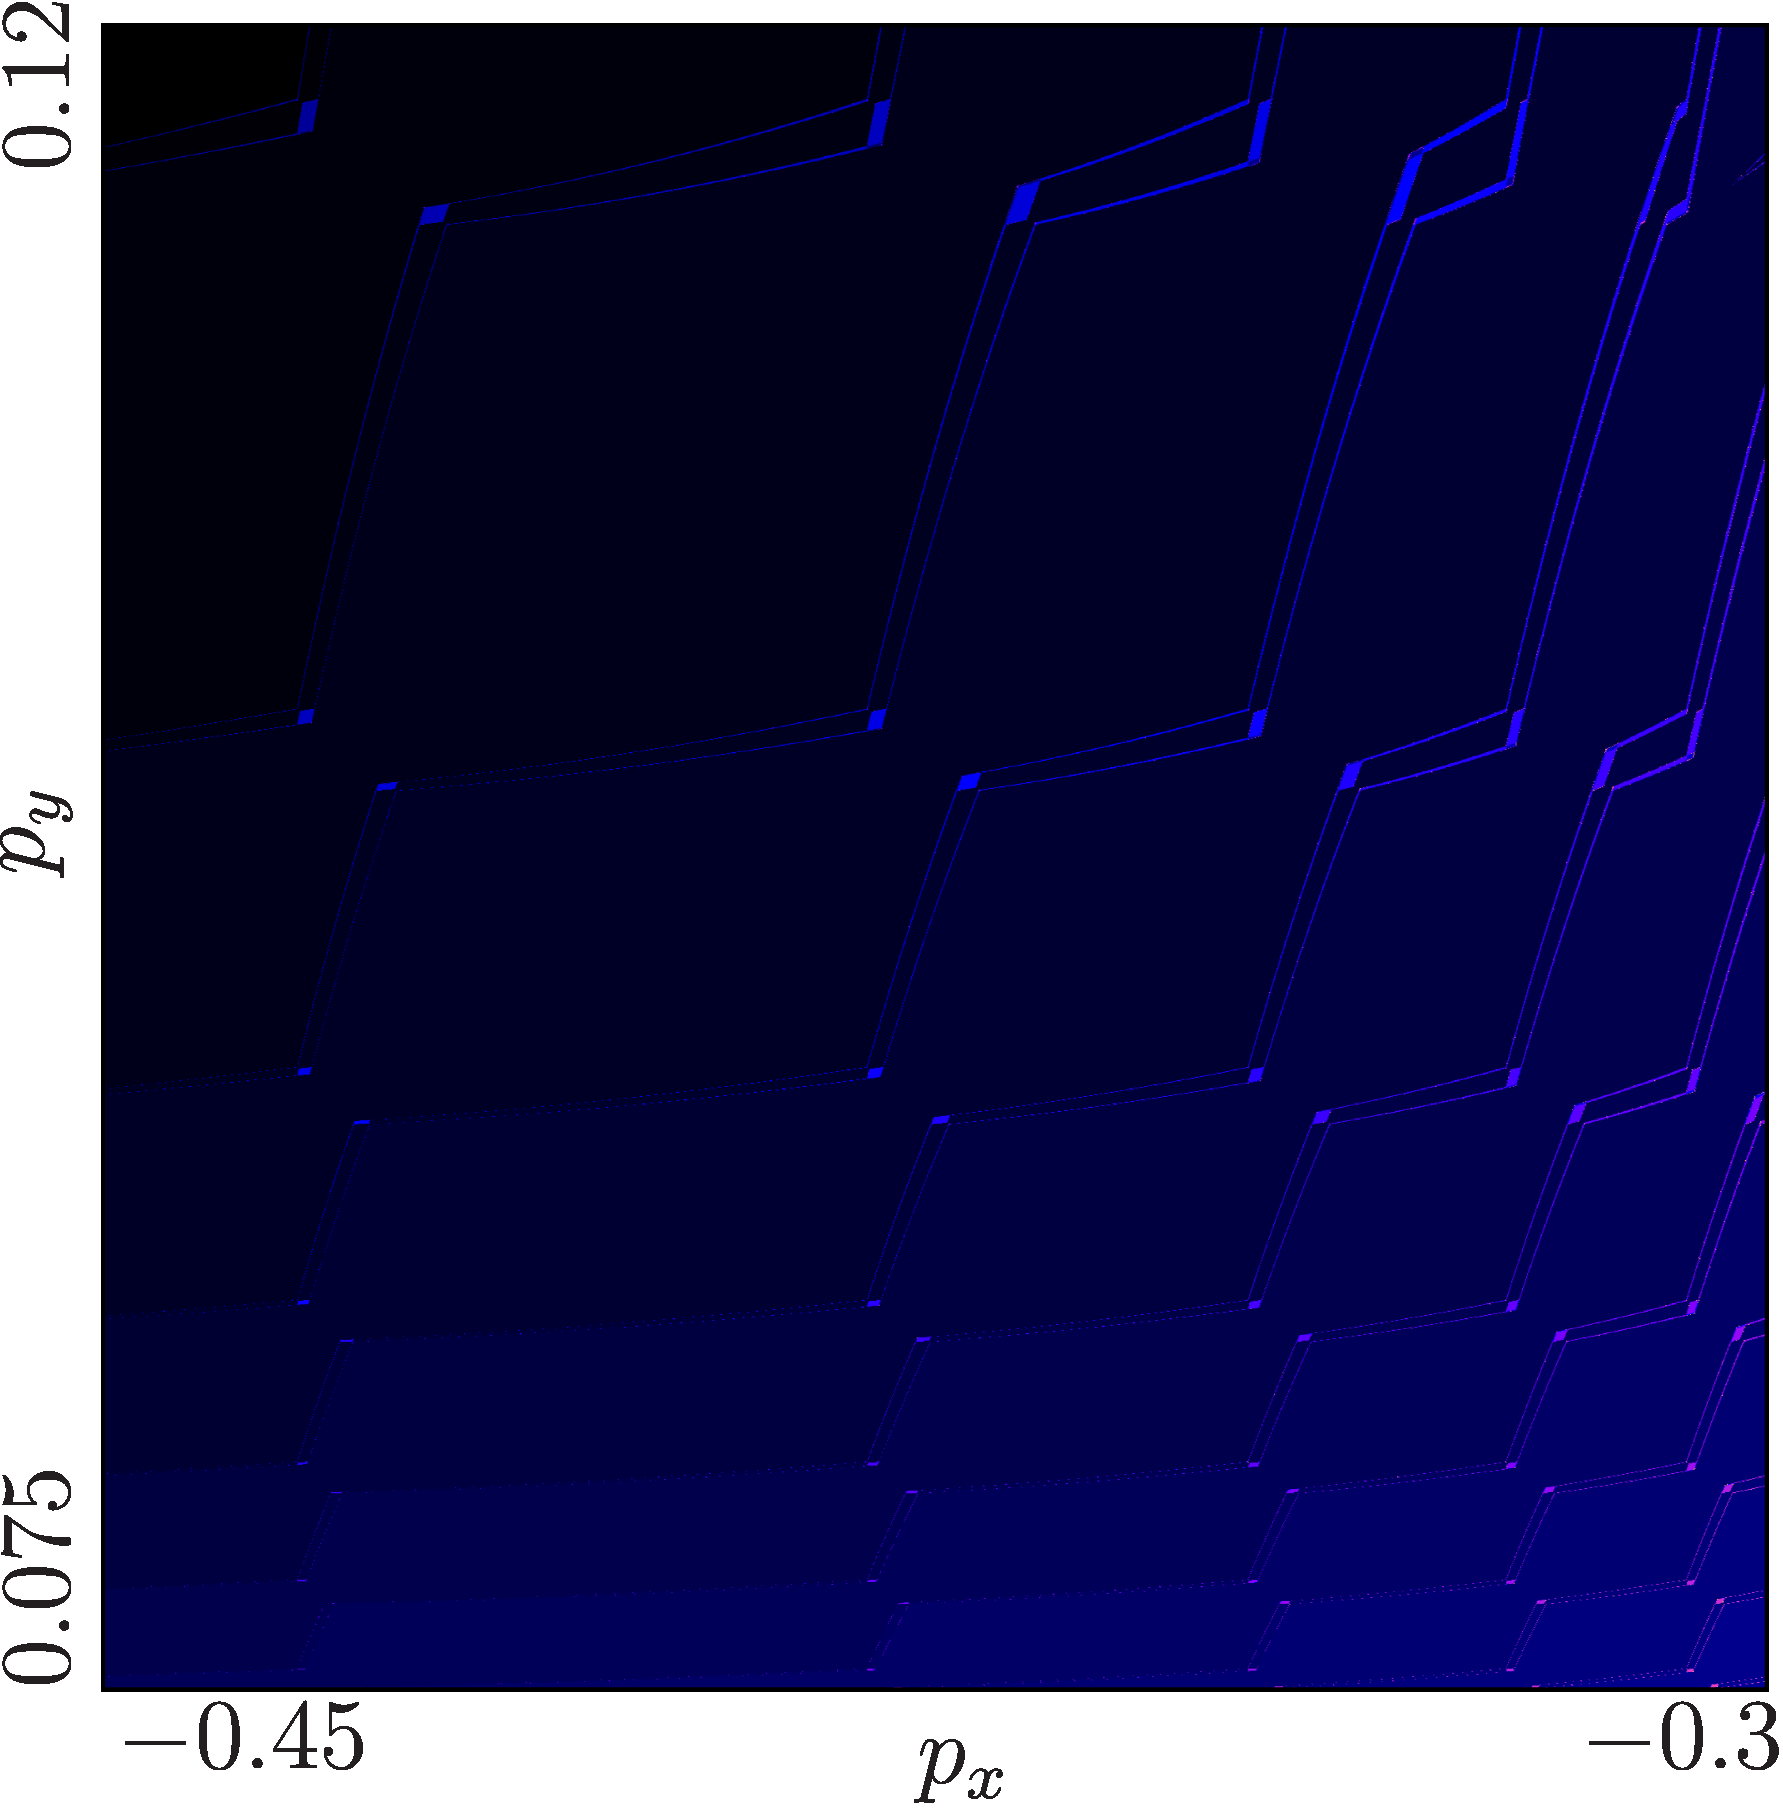
\includegraphics[width=.45 \textwidth]{../Figures/7/7.2b/result.png}
		\label{fig:add.arch.new}
	}
	\caption[Comparison of a skew sawtooth map and the archetypal model function]{
		Comparison of a skew sawtooth map and the archetypal model function.
		(a) shows the skew sawtooth map with the parameters $a_L = 0.5$ and $a_R = 1.5$.
		The function is taken from \Citetitle{simpson2018saw}~\cite{simpson2018saw}.
		(b) shows the archetypal model function with the parameters $a_L = 1, b_L = \frac{1}{2}, c_L = 0.168, g_R\left(\frac{1}{4}\right) = -0.4 ,$ and $g_R\left(\frac{1}{2}\right) = \frac{1}{2} + \frac{1}{40}$.
		\todo{Adjust caption}
	}
	\label{fig:add.saw.vs.arch}
\end{figure}


\todo{From here period-adding-like!}
